\chapter{Estrategias de Testing}
\label{chap:estrategias-de-testing}

\coolquote{
	Probar programas sirve para demostrar la presencia de errores, pero nunca para demostrar su ausencia
}{
	{Edsger W. Dijkstra}
}

El proceso de testing dentro de un proyecto de software es una actvidad que tene como objetivo \ul{verificar} y \ul{validar} que el software cumple con los requisitos especificados.

{El proceso de testing conlleva:\ns
\begin{itemize}
	\item planificación,
	\item diseño,
	\item ejecución de pruebas
	\item evaluación
\end{itemize}}


La gestión de calidad debe garantizar que el proceso de
testing se lleve a cabo de manera eficiente y eficaz.

\section{Tipos de Testing}
\begin{itemize}
	\item Testeo \textbf{unitario}\\
   Testeo de unidades de software individuales
	\item Testeo de \textbf{integración}\\
   Testeo de los interfaces y de la interacción entre las unidades previamente testeadas
	\item Testeo de \textbf{sistema}\\
   Testeo del sistema entero
	\item Testeo de \textbf{aceptación}\\
   Testeo del sistema y los criterios de aceptación previamente establecidos con el cliente
\end{itemize}

\subsection{Testeo Unitario}
Las \textbf{unidades} son Clases/Métodos (en OO), Procedimientos, Módulos o Componentes. Como se definen las unidades depende del diseño, de la criticidad del software (más crítico implica unidades más pequeñas), de la empresa (estrategia), o del tiempo disponible.


Una \textbf{prueba unitaria} (\texttt{unit test}) es una pieza de código escrita por un desarrollador que pone a prueba un pequeño y específico trozo de código.
Es una manera relativamente barata para mejorar la calidad del código producido, pero \textit{NO} es para usuarios, gerentes, jefes de proyectos: està hecha para los programadores.
El programador examina o ejecuta una pequeña
parte de su código, para testear
\ul{la funcionalidad que él o ella piensa que tiene que tener}

\begin{figure}[htbp]
   \centering
   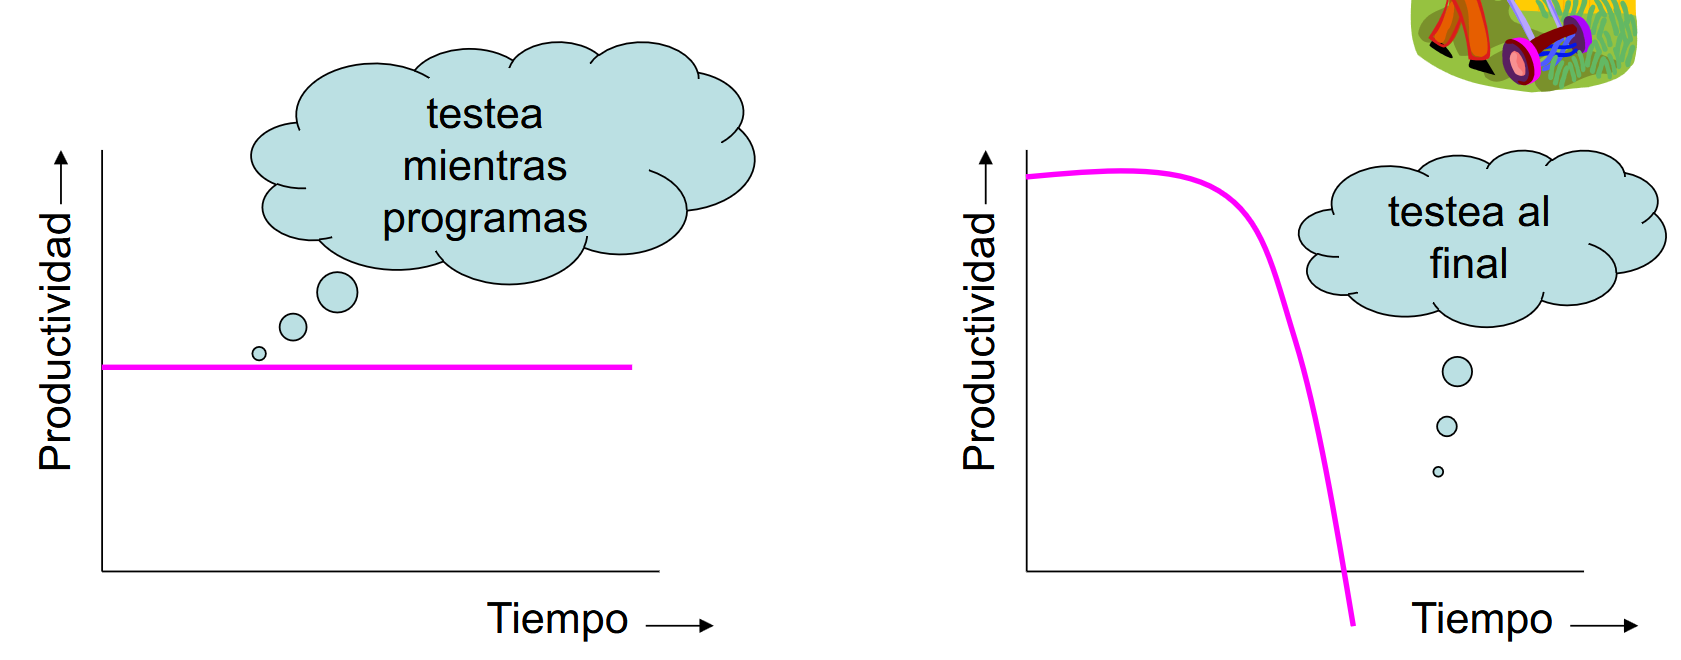
\includegraphics{images/03/unitPostpone.png}
   \caption{Posponer el testeo unitario cuesta mucho tiempo}
   \label{fig:03/unitPostpone}
\end{figure}

\coolquote{
   No es mi trabajo hacer testeo, tenemos un departamento de calidad
}{Bad programmer}

Entonces ¿cuál es el trabajo de un programador? El trabajo de cada programador es \ul{producir código que
funciona y que no contenga ``muchos'' errores}

\subsubsection{JUnit}

\begin{paracol}{2}
	
	\colfill
	\textsc{JUnit} es un framework de testing para Java. \textsc{JUnit} es una herramienta que ayuda a los programadores a escribir pruebas unitarias en Java. \textsc{JUnit} ha sido importante en el desarrollo de la metodología de programación extrema (XP).
	\lstinline|@Test| son los métodos de prueba.
	\begin{itemize}
		\item \lstinline|@BeforeEach| se invoca antes de la ejecución de cada test
		\item \lstinline|@AfterEach| se invoca después de la ejecución de cada test
		\item \lstinline|@BeforeAll| se invoca antes de la ejecución de todos los tests
		\item \lstinline|@AfterAll| se invoca después de la ejecución de todos los tests
		\item[] Estas anotaciones son de \textsc{JUnit 5}, en \textsc{JUnit 4} se usaba \lstinline|@Before| y \lstinline|@After|, además de otras diferencias.
	\end{itemize}
	
	El codigo de testo para una clase \lstinline|MyClass| se pone en una clase \lstinline|TestMyClass|, y el método para testear el método \lstinline|myMethod| se llama \lstinline|testMyMethod|, o algo similar, como \\
	\lstinline|testMyMethodSimple|, \lstinline|testMyMethodAll|, etc.
	\colfill
	\switchcolumn

	\begin{lstlisting}
public class TestDB {
	static private Connection dbConn;
	static private Account acc;
	@BeforeAll
	public static void setUpBeforeAll(){
		dbConn = new Connection("Oracle",15,fred, "f");
		dbConn.connect();
	}
	@AfterAll
	public static void tearDownAfterAll(){
		dbConn.disconnect();
		dbConn = null;
		}
	@BeforeEach
	protected void setUp(){
		acc = new Account();
		}
	@AfterEach
	protected void tearDown(){
		acc = null;
	}
	
	public void testAccountAccess(){
	.../Uses dbConn and acc
	}
	public void testEmployeeAccess(){
		.../Uses dbConn and acc
		}
\end{lstlisting}			
\end{paracol}

\begin{paracol}{2}
	
	\colfill
	En el ejemplo anterior, se muestra un test de una clase \texttt{Account} que tiene una conexión a una base de datos. Se puede ver que se crea una conexión a la base de datos en el método \texttt{setUpBeforeAll} y se cierra en el método \texttt{tearDownAfterAll}. Además, se crea una instancia de la clase \texttt{Account} en el método \texttt{setUp} y se destruye en el método \texttt{tearDown}.
	\colfill
	
	\switchcolumn
	Los metodos son ejecutados en el siguiente orden:
	\ns
 \begin{itemize}
	\item \lstinline|setUpBeforeAll|
	      \begin{itemize}
		      \item \lstinline|setUp|
		            \begin{itemize}
			            \item \lstinline|testAccountAccess|
		            \end{itemize}
		      \item \lstinline|tearDown|
		      \item \lstinline|setUp|
		            \begin{itemize}
			            \item \lstinline|testEmployeeAccess|
		            \end{itemize}
		      \item \lstinline|tearDown|

	      \end{itemize}
	\item \lstinline|tearDownAfterAll|
\end{itemize}
\end{paracol}

\paragraph{Test Suite}
Un test suite es una combinación de clases de prueba que
permite ejecutar todas las pruebas contenidas en dichas
clases a la vez en un orden establecido.
Para crear una Test suit se debe:
\begin{itemize}
	\item Crear una clase Java
	\item Anotar la clase con la etiqueta \lstinline|@RunWith(JUnitPlatform.class)|
	\item Indicar las clases que forman parte de la suite con la
etiqueta \lstinline|@SelectClasses|, o \lstinline|@SelectPackages|
\end{itemize}

A continuación, se muestra un ejemplo de código de la test suite \lstinline|AllTests| que
agrupa las pruebas de las clases \lstinline|LargestTest| y \lstinline|MiClaseDeTest|.

\begin{lstlisting}
	
	import org.junit.platform.runner. JUnitPlatform;
	import org. junit.platform.suite.api.SelectClasses;
	import org.junit.runner.RunWith;
	
	@RunWith (JUnitPlatform.class)
	@SelectClasses ({ LargestTest.class, MiClaseDeTest.class } )
	public class AllTests {
		
		}
\end{lstlisting}

Cuando lancemos a ejecución el test suite \lstinline|AllTests| se ejecutarán primero las
pruebas de la clase \lstinline|LargestTest|, y a continuación las pruebas de la clase
\lstinline|MiClaseDeTest|.

\paragraph{Testeo Parametrizado}
Los test parametrizados posibilitan ejecutar un test con
diferentes argumentos.
Estos tests son declarados como los tests
básicos (\lstinline|@Test| methods) pero usan la etiqueta
\lstinline|@ParameterizedTest|.

Es necesario declarar al menos una fuente que proporcionará
los argumentos para cada invocación del método.
Esto se puede hacer con la anotación \lstinline|@ValueSource| y un
array de valores literales,
pero Existen también otras formas de hacerlo, por ejemplo, con
valores de un fichero csv utilizando la anotación
\lstinline|@CsvFileSource|.

\begin{lstlisting}
	@ParameterizedTest
	@ValueSource (strings = { "racecar", "radar", "able was I ere I saw elba" } )
	void palindromesTest (String candidate) {
		assertTrue (StringUtils.isPalindrome (candidate) );
	}
\end{lstlisting}

\begin{paracol}{2}
	\colfill
\begin{lstlisting}[caption={Ejemplo de clase Factorial}]
public class Factorial {
	public static int factorial(int n) {
		if (n < 0) {
			throw new IllegalArgumentException("n must be nonnegative");
		}
		int result = 1;
		for (int i = 1; i <= n; i++) {
			result *= i;
		}
		return result;
	}
}
\end{lstlisting}
\colfill

\switchcolumn

\begin{lstlisting}[caption={Ejemplo de clase de test de  Factorial}]

public class FactorialTest {
	@Test
	public void testFactorialOfZero() {
		assertEquals(1, Factorial.factorial(0));
	}

	@Test
	public void testFactorialOfOne() {
		assertEquals(1, Factorial.factorial(1));
	}

	@Test
	public void testFactorialOfPositiveNumber() {
		assertEquals(24, Factorial.factorial(4));
	}

	@Test(expected = IllegalArgumentException.class)
	public void testFactorialOfNegativeNumber() {
		Factorial.factorial(-1);
	}
}
	
\end{lstlisting}
\end{paracol}

\begin{lstlisting}
@RunWith(Parameterized.class)
public class FactorialParametrizedTest {
	private int input;
	private int expected;

	public FactorialParametrizedTest(int input, int expected) {
		this.input = input;
		this.expected = expected;
	}

	@Parameterized.Parameters
	public static Collection<Object[]> data() {
		return Arrays.asList(new Object[][] {
				{ 0, 1 }, { 1, 1 }, { 2, 2 }, { 3, 6 }, { 5, 120 }, { 9, 362880 },
				{ 12, 479001600 }, { -1, 1 }

		});

	}

	@ParametrizedTest
	@MethodSource("data")
	public void testFactorial() {
		assertEquals(expected, Factorial.factorial(input));
	}

}
\end{lstlisting}
\subsection{Testeo de Integración}

\begin{definition}
	[Testeo de Integración]
	El testing de las interfaces y la
	interacción entre las unidades previamente testeadas
	mientras que se ensambla el sistema entero
\end{definition}

\begin{itemize}
	\item ¿Qué componentes son el foco del testeo de integración?
	\item ¿En qué orden vamos a testear las interfaces?
	\item ¿Qué técnicas utilizamos para testear las interfaces?
\end{itemize}

Hay tres estrategias:
\begin{enumerate}
	\item \textbf{Big Bang} (todos los componentes a la vez)
	\item \textbf{Bottom-up} (de abajo hacia arriba)
	\item \textbf{Top-down} (de arriba hacia abajo)
\end{enumerate}

\begin{figure}[htbp]
	\centering
	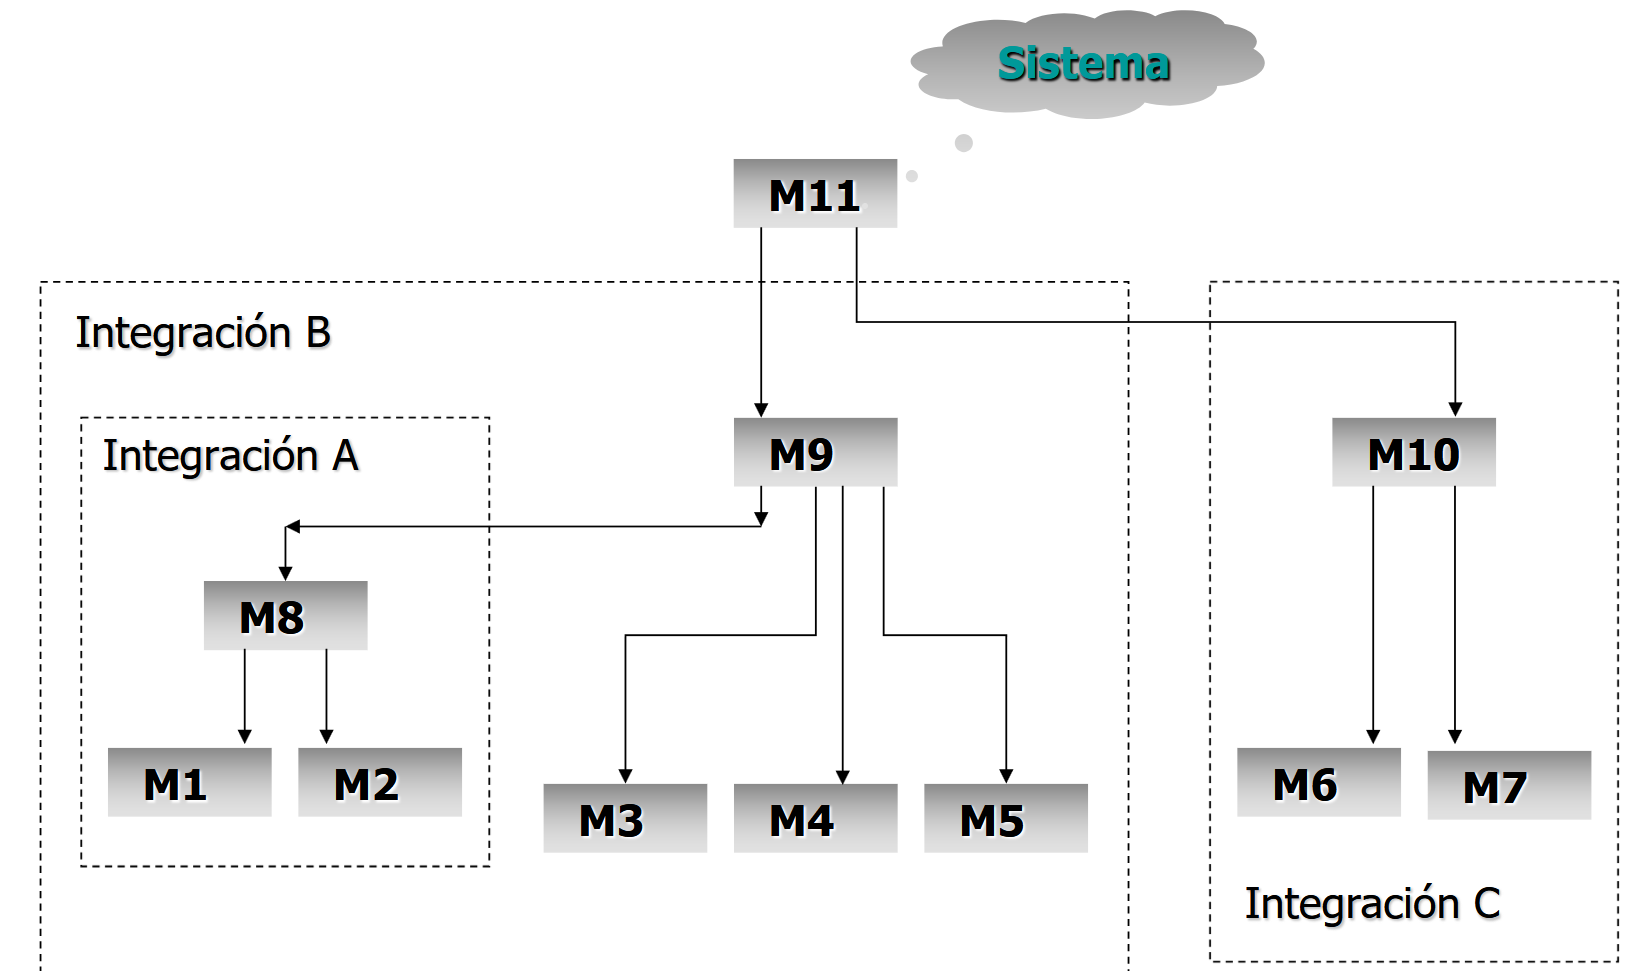
\includegraphics{images/03/bottomup.png}
	\caption{Arbol de dependencia y Bottom-up testing}
	\label{fig:03/bottomup}
\end{figure}

Para hacer el testing \textit{bottom-up} necesitamos \textbf{drivers}.
Un driver es un programa que invoca un componente bajo testeo, por ejemplo, para simular un componente de un nivel superior cuyo código todavía no está disponible (está todavía en desarrollo).
\note{Por ejemplo un driver puede simular el componente M9 che invoca M8, si estamos testeando M8.}

\begin{figure}[htbp]
	\centering
	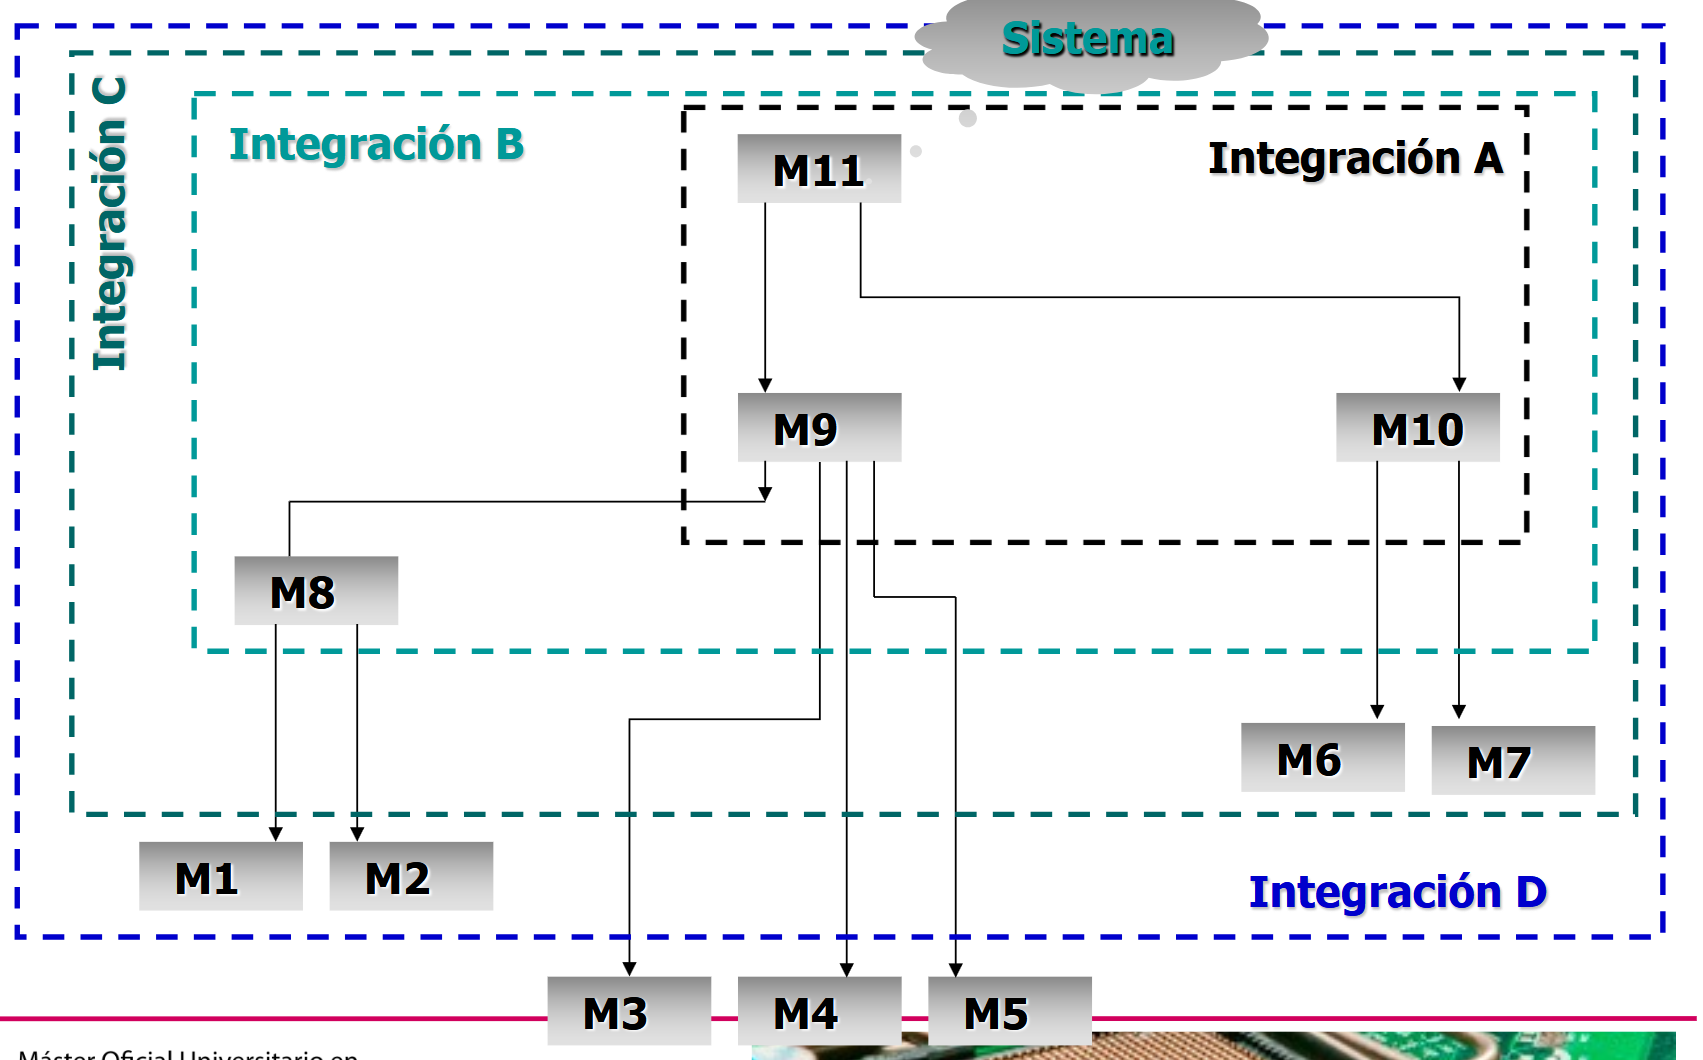
\includegraphics{images/03/topdown.png}
	\caption{Top-down testing}
	\label{fig:03/topdown}
\end{figure}

Para hacer el testeo de integración de manera \textit{top-down}, se
necesita dobles, que simulan componentes de un nivel inferior (``Stub'', ``dummy'', ``fake'', ``mock'').
\note{Si estamos testeando M8, podemos sostituir M1 y M2 con mocks}
\ns

El \textit{Big Bang} testing se utiliza solo para sistemas pequeños, ya que es muy difícil de manejar en sistemas grandes.


\subsubsection{Top-Down}
\begin{lstlisting}
	public float calculaSalarioNeto(float salarioBruto) throws BRException {
		float retencion = 0.0f;
		if (salarioBruto < 0) {
			throw new BRException("El salario bruto debe ser positivo");
		}
		// PROXY HERE!
		ProxyAeat proxy = getProxyAeat();
		List<TramoRetencion> tramos;
		try {
			// Invoke the emulated function!
			tramos = proxy.getTramosRetencion();
		} catch (IOException e) {
			throw new BRException("Error al conectar al servidor de la AEAT", e);
		}
		for (TramoRetencion tr : tramos) {
			if (salarioBruto < tr.getLimiteSalario()) {
				retencion = tr.getRetencion();
				break;
			}
		}
		return salarioBruto * (1 - retencion);
	}
	
	public class MockProxyAeat extends ProxyAeat {
		boolean lanzarExcepcion;
	
		public MockProxyAeat(boolean lanzarExcepcion) {
			this.lanzarExcepcion = lanzarExcepcion;
		}
	
		@Override
		public List<TramoRetencion> getTramosRetencion()
				throws IOException {
			if (lanzarExcepcion) {
				throw new IOException("Error al conectar al servidor");
			}
			List<TramoRetencion> tramos = new ArrayList<TramoRetencion>();
			tramos.add(new TramoRetencion(1000.0f, 0.0f));
			tramos.add(new TramoRetencion(1500.0f, 0.16f));
			tramos.add(new TramoRetencion(Float.POSITIVE_INFINITY, 0.18f));
			return tramos;
		}
	}
\end{lstlisting}

\begin{lstlisting}[caption={Utilizar en el testing}]
class TestableEmpleado extends Empleado {
	ProxyAeat proxy;

	public void setProxyAeat(ProxyAeat proxy) {
		this.proxy = proxy;
	}

	@Override
	ProxyAeat getProxyAeat() {
		return proxy;
	}
}

TestableEmpleado empleadoTest;

@BeforeEach
public void setUpClass() {
	empleadoTest = new TestableEmpleado();
	empleadoTest.setProxyAeat(new MockProxyAeat(false));
	empleadoTestFail = new TestableEmpleado();
	empleadoTestFail.setProxyAeat(new MockProxyAeat(true));
}

@Test
public void testCalculaSalarioNeto1() throws BRException {
	float resultadoReal = empleadoTest.calculaSalarioNeto(2000.0f);
	float resultadoEsperado = 1640.0f;
	assertEquals(resultadoEsperado, resultadoReal, 0.01);
}
	
\end{lstlisting}
\subsubsection{Mockito}
Mockito es un framework de testing para Java que permite crear objetos simulados (mocks) de clases y interfaces. Mockito se utiliza para simular objetos que son necesarios para realizar pruebas unitarias. Se puede integrar con JUnit para realizar pruebas unitarias en Java. 
En las slides se muestran ejemplos de cómo utilizar Mockito.

Mockito es muy comodo para implementar el testeo de integración de manera \textit{top-down}.
% TODO Parte 2 y 3

\begin{lstlisting}
public class CalculatorServiceImpl implements CalculatorService {
   private DataService dataService;

   public double calculateAverage() {
      int[] numbers = dataService.getListOfNumbers();
      double avg = 0;
      for (int i : numbers) {
         avg += i;
      }
      return (numbers.length > 0) ? avg / numbers.length : 0;
   }

   public void setDataService(DataService dataService) {
      this.dataService = dataService;
   }
}

@RunWith(MockitoJUnitRunner.class)
public class CalculatorServiceTest {
	// Automatically set data service to point to mock
   @InjectMocks
   private CalculatorServiceImpl calculatorService;
   @Mock
   private DataService dataService;

   @Test
   public void testCalculateAvg_simpleInput() {
		// define what to yield when the mock methods are invoked
      when(dataService.getListOfNumbers()).thenReturn(new int[] { 1, 2, 3, 4, 5 });
      assertEquals(3.0, calculatorService.calculateAverage(), .01);
   }

   @Test
   public void testCalculateAvg_emptyInput() {
      when(dataService.getListOfNumbers()).thenReturn(new int[] {});
      assertEquals(0.0, calculatorService.calculateAverage(), .01);
   }

   @Test
   public void testCalculateAvg_singleInput() {
      when(dataService.getListOfNumbers()).thenReturn(new int[] { 1 });
      assertEquals(1.0, calculatorService.calculateAverage(), .01);
   }
}
\end{lstlisting}

\section{Testeo de Sistema}
Se verifica que se cumple los requisitos especificados, es decir, que el sistema realiza correctamente todas las funciones que se han detallado en las especificaciones dadas por el usuario del sistema.

Es necesario automatizar las prubas, y por esto se utilizan herramientas como \textit{Selenium}, que permite automatizar pruebas en navegadores web: en este caso, hablamos de pruebas de \textbf{funcionalidad}.

Para testar el \textbf{rendimiento} (tiempo de respuesta, carga, memoria.) se utilizan herramientas como \textit{JMeter} o \textit{NeoLoader}.

Otros aspectos importantes que el testeo debe cubrir son \textbf{Seguridad} y \textbf{Usabilidad}.

\labelitemize{Seguridad}{
\begin{itemize}
	\item Evaluar la capacidad del sistema de software de prevenir
	acceso no autorizado.
	\item Casos de test Npicos examinan funciones como:
	\begin{itemize}
		\item logon, logoff
		\item cambio de permisos
		\item chequeo de contraseñas
		\item caducidad de contraseñas
	\end{itemize}
\end{itemize}
}

\labelitemize{Usabilidad}{
 \begin{itemize}
	\item Usabilidad es el conjunto de características que influyen en el esfuerzo requerido para el aprendizaje, el uso, la preparación de entradas y la interpretación de salidas del programa por parte de un conjunto de usuarios dados
	      \begin{itemize}
		      \item Memorabilidad (el esfuerzo del usuario para comprender el software
		            una vez ya había aprendido a usarlo)
		      \item Facilidad de aprendizaje (el esfuerzo del usuario para aprender el
		            software)
		      \item Operabilidad/eficiencia (el grado en que el usuario puede ejecutar las
		            tareas que son objeDvo del software)
		      \item Eficacia (el grado en que el usuario comete errores)
		      \item Atractivo (ergonomía, colores, formas, )
	      \end{itemize}

	\item La major manera da evaluar si un producto es usable es involucrandolo a los usuarios, que son los que deciden si el producto es usable o no.
\end{itemize}
}


\section{Testeo de aceptación}
Esto testeo es dirigido a los criterios de aceptación
previamente establecidos con el cliente. Se puede hacer de manera manual o automatizada.

{Es importante recordar dos axiomas:\ns
\begin{itemize}
	\item Axioma de \textbf{decomposición}: Aunque se ha testeado un sistema adecuadamente, eso no significa que se ha testeado adecuadamente sus componentes.
	\item Axioma de \textbf{anticomposición}: Testear cada uno de los componentes de un sistema por separado no necesariamente significa que el sistema entero está testeado adecuadamente.
\end{itemize} 
}
\subsection{Regresión}
Testeo que se necesita hacer después de cambios en el
software para asegurar que no se ha introducido defectos.

\ul{El testeo de \textbf{regresión} se tiene que automatizar} por el simple hecho de que el testeo de regresión manual \textit{NO SE HACE}.

\section{Gestión de Defectos, métricas y mas}

{El proceso de clasificación de defectos incluye tres fases:\ns
\begin{enumerate}
	\item \textbf{Detección} de defectos
	\item \textbf{Investigación} de defectos
	\item \textbf{Resolución} de defectos
\end{enumerate}}

\vspace{1em}

\note{
	Para cada defecto tenemos que registrar algunas informaciones.
\begin{itemize}
	\item \textbf{Actividad} (que estábamos haciendo cuando encontramos el fallo)
	\item \textbf{Fase del proyecto} (en que estábamos cuando encontramos el fallo)
	\item \textbf{Repetitividad} (¿se puede repetir el error?)
	\item \textbf{Síntoma} (fallo del sistema, mensaje de error, entrada no aceptado, resultado
incorrecto, etc.)
	\item \textbf{Causa} (nuestro producto, componente externo, usuario, etc.)
	\item \textbf{Origen} (especificación de requisitos, diseño, programación, etc.)
	\item \textbf{Impacto} (misión: crítico, medio, …; en la planificación; para el cliente, etc.)
\end{itemize}
}

\subsection{Métricas}


 Las métricas son observaciones cuantitativas para:
\begin{itemize}
	\item Informar sobre el \textbf{progreso del proyecto} de testeo
\note{\begin{itemize}
	\item ¿Qué tareas han terminado en tiempo?
	\item ¿Qué tareas han terminado antes?
	\item ¿Qué tareas han tenido retraso?
	\item ¿Cómo vamos siguiendo la planificación?
	\item Si no vamos bien, ¿cuáles son las razones?
	\item ¿Qué productividad ha tenido persona/equipo X?
\end{itemize}}
	\item Informar sobre la \textbf{calidad del software}
	\note{\begin{itemize}
		\item ¿Podemos parar el testeo?
	\item ¿Podemos entregar producto?
	\item ¿Hemos resueltos todos los defectos?
	\item ¿Cómo estamos gesHonando los defectos?
	\item ¿Cuántos defectos hemos encontrado por: subsistema,
	origen, causa, severidad, etc\dots?
	\end{itemize}}
	\item Informar sobre la \textbf{calidad del testeo}
	\note{\begin{itemize}
		\item ¿Estamos haciendo los tests necesarios?
		\item ¿Están siendo efectivos los tests?
		\item ¿Estamos utilizando los casos de prueba adecuados?
		\item ¿Necesitamos tener en cuenta diferentes casos de prueba?
	\end{itemize}}
\end{itemize}

\subsubsection{Cobertura}

La cobertura del testeo es una métrica importante para evaluar la calidad del testeo. La cobertura del testeo es la medida de la cantidad de código que ha sido ejecutado por los tests, especialmente en lo que se refiere a \textbf{instrucciones}, \textbf{decisiones} y \textbf{condiciones} (múltiples).\\
Pero puede referirse también a la cobertura de los requisitos, de los casos de uso, de los casos de prueba, etc.

\begin{lstlisting}[caption={Con 1 test donde \lstinline|x==y| se cubre todo el codigo, pero no todas las decisiones. En efecto, el defecto ocurre cuando \lstinline|x!=y|}]
	int foo_3 ( ) {
		int* p = NULL;
		int x;
		if (x==y) {
			p = &x;
		}
		*p = 123;
	}
\end{lstlisting}
\begin{itemize}
	\item $G =$ grafo de flujo de control
	\item $A =$ cantidad de arcos en G
	\item $N =$ cantidad de nodos en G
	\item $V(G) = A - N + 2$
\end{itemize}

Complejidad ciclomática $V(G)$ es una aproximación de la cantidad de los casos de test necesarios para cobertura de decisiones.

Está matemáticamente demostrado que $100\%$ cobertura de decisiones se puede hacer con $\leq V(G)$ tests.\\
Sin embargo, se pueden elegir $V(G)$ caminos que NO consiguen $100\%$ de cobertura de decisiones!

Se tiene que interpretar las métricas de cobertura con cuidado:
cobertura alta no dice mucho, pero si es baja hay un problema.

\begin{align}
	PDD &= \textit{Porcentaje de Detección de Defectos}\\
	PDD &= \frac{\#\{\textit{defectos encontrados durante el testeo}\}}{\#\{\textit{defectos encontrados}\}}\times 100
\end{align}
\subsection{Mutación}

La mutación es una técnica de testing que consiste en introducir errores en el código fuente para ver si los tests son capaces de detectarlos. Se puede utilizar para evaluar la calidad de los tests.

\subsection{Organización del testing}
Se puede dedicar un equipo de testo integrado, con un jefe, o se puede haber que desarrolladores y testeadores son las mismas personas y no hay testeadores a tiempo completo.
La ventaja de tener un equipo de testeo es que se puede tener una visión más objetiva del software, ya que los testeadores no han desarrollado el software; al contrario, si los desarrolladores hacen el testeo, no tienen que comunicar con los testeadores, y conocen el software.

Otra tecnica de organización es \textit{Outsourcing}, que consiste en contratar una empresa externa para hacer el testeo. La ventaja es que se puede tener una visión más objetiva del software, y se puede tener acceso a expertos en testeo. La desventaja es que se puede tener problemas de comunicación, y que se puede tener problemas de confidencialidad.

